\documentclass{beamer}
\usetheme{Pittsburgh} 
%\documentclass{article}

\usepackage[utf8]{inputenc}
\usepackage{default}
%\usepackage{natbib}
\usepackage{graphicx}
\usepackage{listings}
%\usepackage{fontspec}
\DeclareFontShape{OT1}{cmtt}{bx}{n}{<5><6><7><8><9><10><10.95><12><14.4><17.28><20.74><24.88>cmttb10}{}

\lstset{language=C++,
                basicstyle=\ttfamily\footnotesize,
                keywordstyle=\color{blue}\ttfamily,
                stringstyle=\color{red}\ttfamily,
                commentstyle=\color{green}\ttfamily,
                morecomment=[l][\color{magenta}]{\#}}

%IMAGE TEMPLATE               
%\begin{figure}[ht!]
%\centering
%\includegraphics[width=90mm]{fixed_dome1.jpg}
%\caption{A simple caption}
%\label{overflow}
%\end{figure}
                
\begin{document}

\title{Interfaces for Youbot-py}
\author{
  Naazare, Menaka \texttt{mnksnz@gmail.com}
  \\ \and
  Quignon, Christophe
  \texttt{cuignon@gmail.com}
  \\ \and
  David Iloube
  \texttt{%mailadress
  }
}
\institute{Hochschule Bonn Rhein Sieg}
\date{\today}

\begin{frame}
\titlepage
\end{frame}

%CONTENTS
%
%PROBLEM
%REQUIRERMENTS
%DESIGN
%CODE
%TESTING

%
%boostpython
%c++
%pyhton

%
%ROSCODE in py move()
%
%Define example interface move()
%find the matching functions ind youbot-py
%find corresponding functions in the youbot driver
%define missing interfaces
%implement them
%
\begin{frame}
\frametitle{Motivation}
\framesubtitle{}
C++ is complicated and cumbersome because of its age. Python is readable and concise.\\
The basic youbot driver is written in C++, so we are going to access the Youbot through a Python interface.\\[\baselineskip]
In this mini project we aim to test the youbot-py with our own interface and improve the library with missing parts.  
\end{frame}


\begin{frame}
\frametitle{Approach}
\framesubtitle{}
  \begin{enumerate}   \item PROBLEM
   \begin{itemize}  \item define example interface (like \texttt{move(x, y, z)})   \end{itemize}
   \item REQUIREMENTS
   \begin{itemize}    
    \item find the matching functions in youbot-py 
    \item find corresponding functions in the youbot driver 
   \end{itemize}
   \item DESIGN \begin{itemize} \item define missing interfaces \end{itemize}
   \item CODE
   \item TEST
  \end{enumerate}

\end{frame}

%ORDER
%abstract->concrete
%1 structural diagram & 1 behavioural diagram
%use case
%State diagram
%Components
%CLass Diagram


\begin{frame}
 \frametitle{Problem}
 \framesubtitle{State Diagram}

 \begin{figure}[ht!]
  \centering
  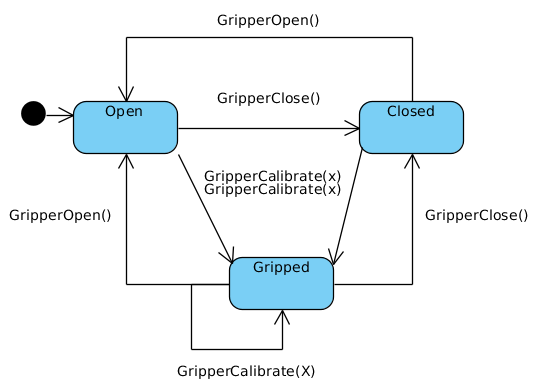
\includegraphics[width=90mm]{img/statechart.png}
  \caption{}
  \label{State Diagram Of The Gripper}
  \end{figure} 
 \end{frame}
 
 
 \begin{frame}
 \frametitle{Problem}
 \framesubtitle{Transition Diagramm}

 \begin{tabular}{ l | c c c }
            & Opened & Closed & Gripped \\ \hline
  Opened    & - & g-hold() & g-calibrate(x, y) \\
  Closed    & g-release & - & g-calibrate(x, y) \\
  Gripped   & g-select() & g-hold() & g-calibrate(x, y)
  \end{tabular}

\end{frame}

\begin{frame}
 \frametitle{Design}
 \framesubtitle{Components Diagram}
%MANDATORY
  \begin{figure}[ht!]
  \centering
  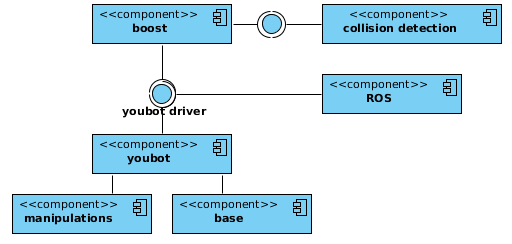
\includegraphics[width=90mm]{img/components.png}
  \caption{}
  \label{Component Diagram}
  \end{figure} 
\end{frame}


\begin{frame}
 \frametitle{Design}
 \framesubtitle{Class Diagram}
  \begin{figure}[ht!]
  \centering
  \includegraphics[width=90mm]{uml.jpeg}
  \caption{}
  \label{overflow}
  \end{figure}
 
\end{frame}


\begin{frame}[fragile]
 \frametitle{Code}
 \framesubtitle{binding.h}
\begin{lstlisting}[language=C++]
namespace YOUBOTPYTHON{
using namespace boost::python;

class PyRobotArm;

class Arm {
public:
    Arm();
    uint8_t calib;
    /*[..]*/

    /*Miniproject additions*/
    Gripper();
    bool setConfigurationParameter(const object& o);
    open();
    close();
    /*for later implementation*/
    /*object getGripperBar1();
    object getData(const object& o);
    bool setData(const object& o);
    object getConfigurationParameter(const object& o);	
    object getGripperBar2();
    bool setValueToMotorContoller();
    object retrieveValueFromMotorContoller(const object& o);
    */
};
\end{lstlisting} 
\end{frame}

\begin{frame}[fragile]
 \frametitle{Code}
 \framesubtitle{BINDING.CPP}
\begin{lstlisting}[language=C++]
BOOST_PYTHON_MODULE(youbot)
{
    using namespace boost::python;
    numeric::array::set_module_and_type("numpy", "ndarray"); 
    import_array();
    class_<YOUBOTPYTHON::Arm, boost::noncopyable>("arm",init<>())

      .def("CalibrateStandard", &Arm::startcalib)
      /*[..]*/
      .def("Reset", &Arm::Reset);

      /*Miniproject additions*/
      .def("getData", &Gripper::getData)
      .def("setData", &Gripper::getData)
      .def("open", &Gripper::open)
      .def("close", &Gripper::close)
      .def("setConfigurationParameter", &Gripper::setConfigurationParameter)
      /*for later implementation*/
      /*.def("getConfigurationParameter", &Gripper::getConfigurationParameter)
      .def("getGripperBar1", &Gripper::getGripperBar1)
      .def("getGripperBar2", &Gripper::getGripperBar2)
      .def("setValueToMotorContoller", &Gripper::setValueToMotorContoller)
      .def("retrieveValueFromMotorContoller", &Gripper::retrieveValueFromMotorContoller)
      */
\end{lstlisting} 
\end{frame}


%\begin{frame}
%        \frametitle{Reference}
%        \bibliographystyle{amsalpha}%amsalpha
%        \bibliography{precoursebib.bib} 
%\end{frame}


%\begin{lstlisting}[language=C++]


\end{document}
